\subsection{GraphGPS with HIG}
GraphGPS is by design a highly malleable model, which allows for easy additions to the code. Thus we implemented HiG in a section of GraphGPS.

\begin{figure}[ht]
    \centering
    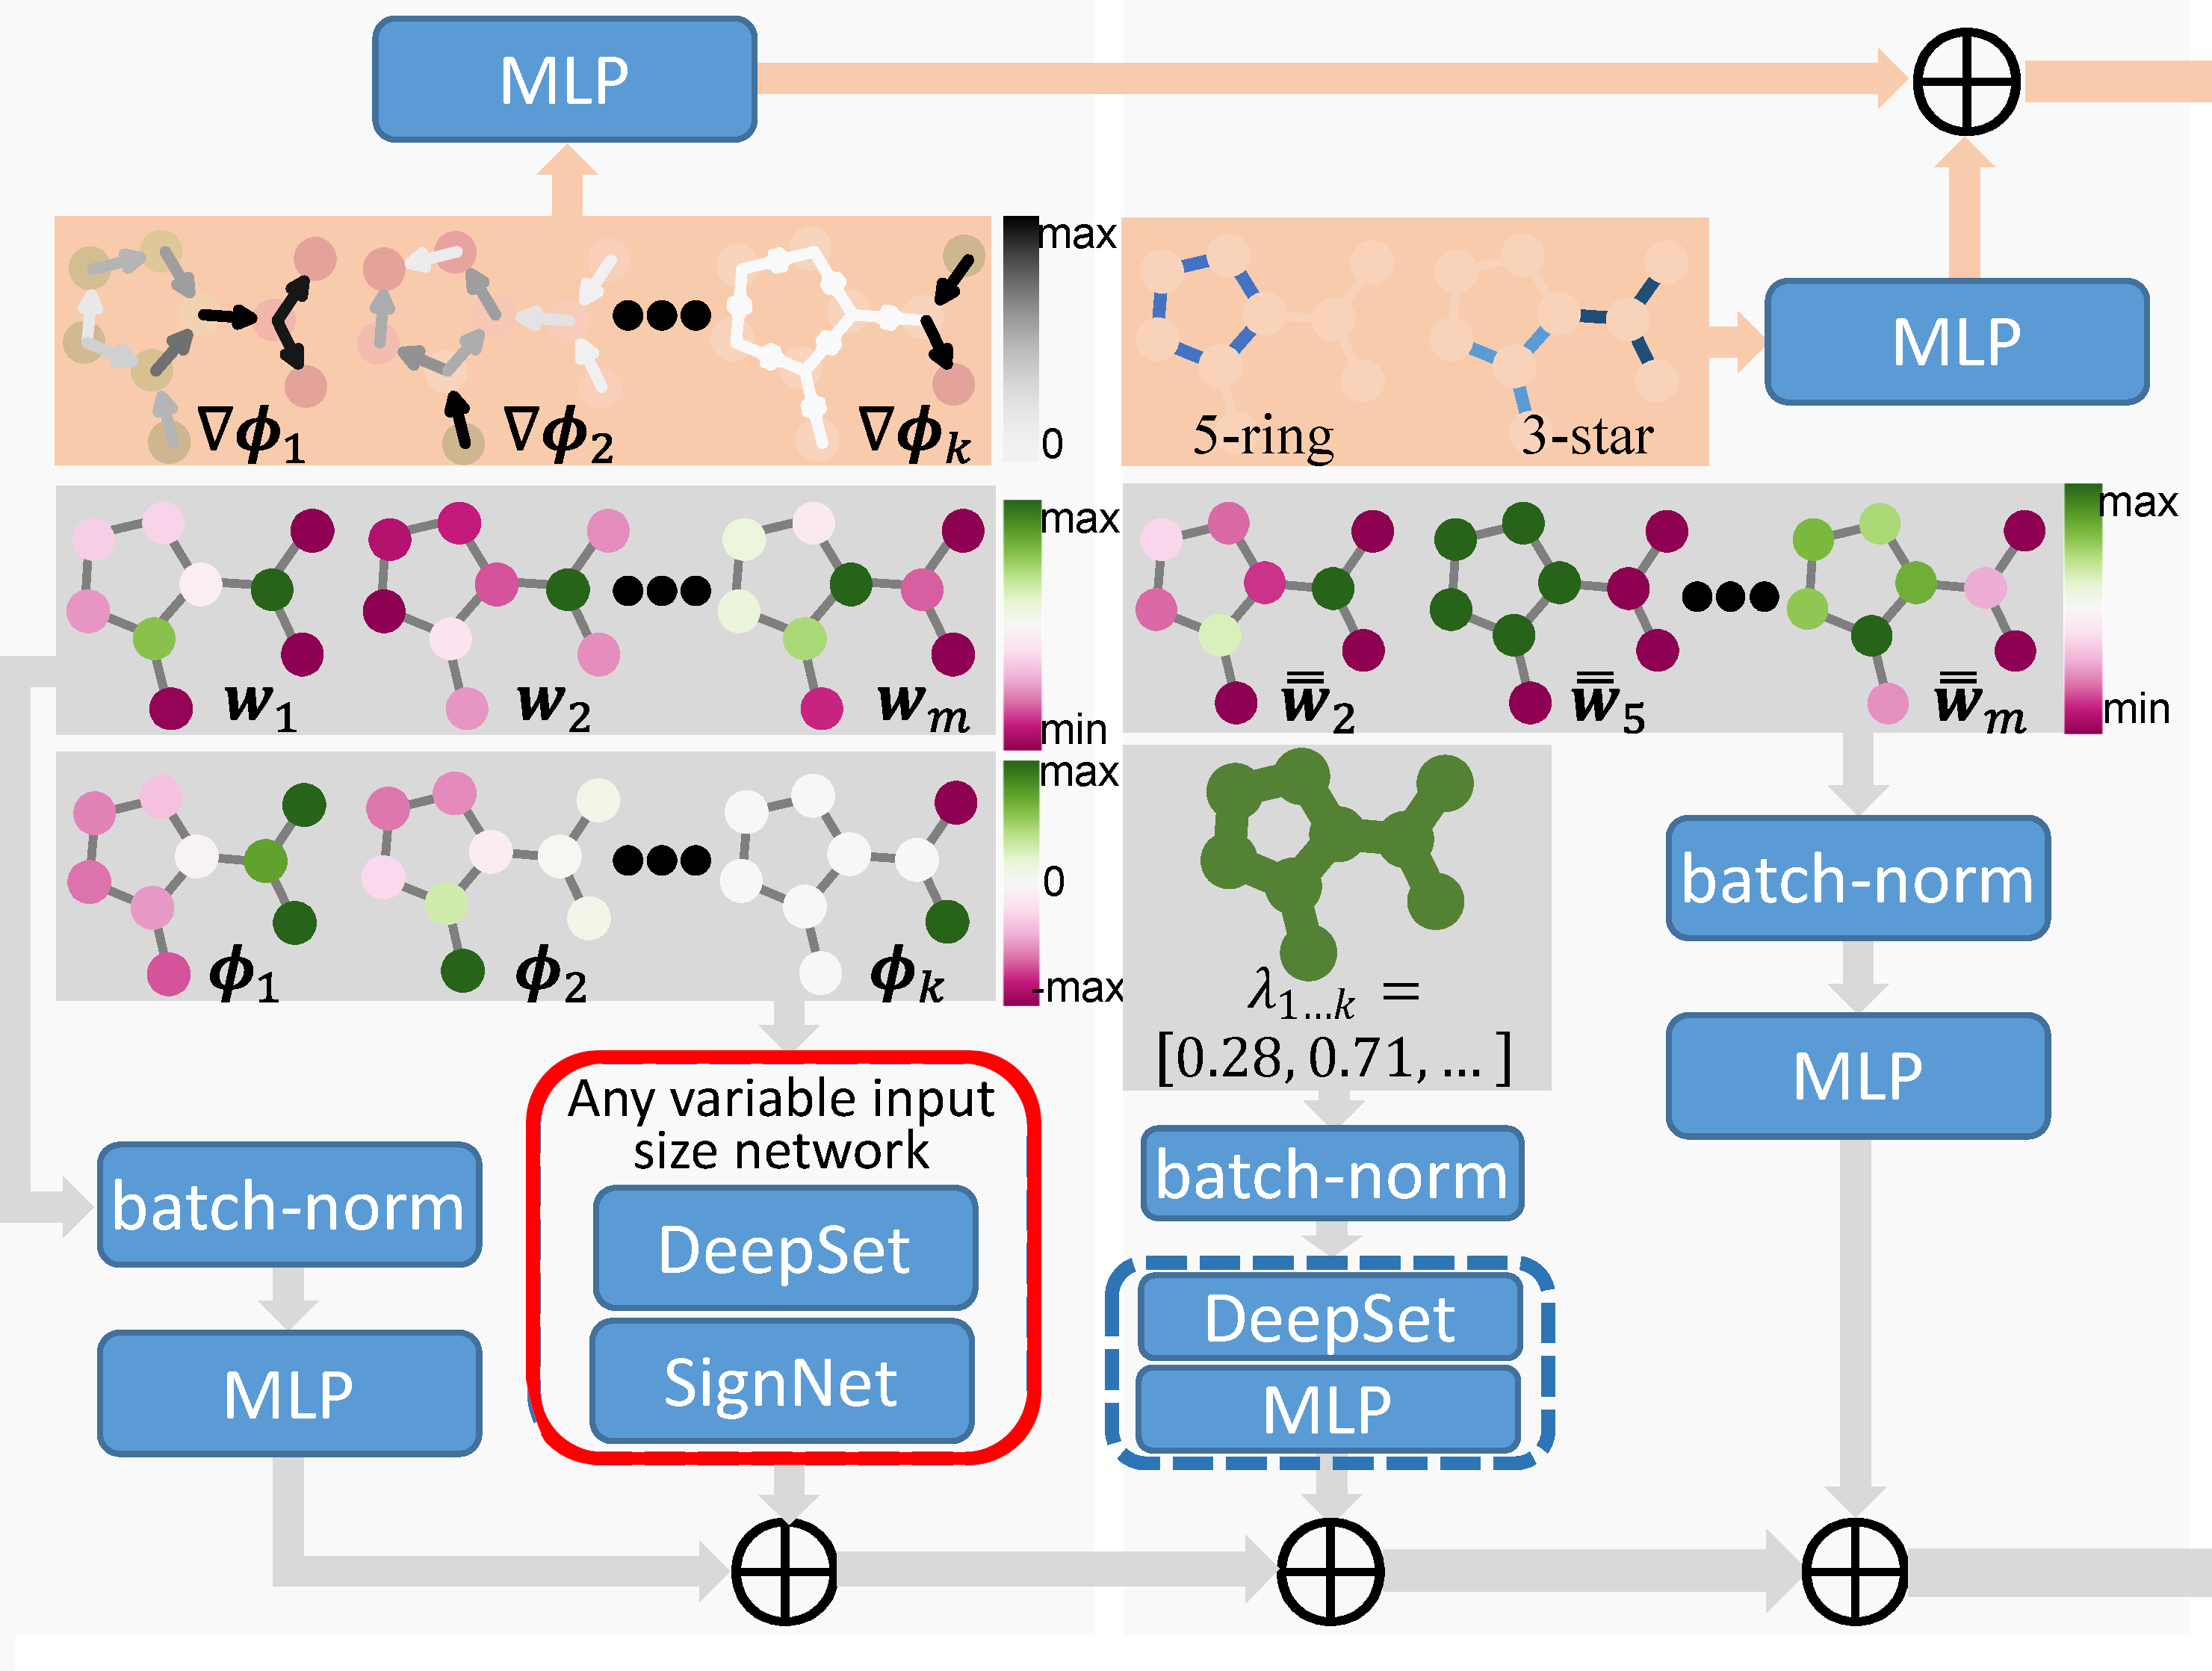
\includegraphics[scale=0.2]{tex/res/gps_hig_position.png}
    \caption{Position of our approach in the architecture}
    \label{fig:gps-hig-position}
\end{figure}

\subsubsection{Implementation}
\begin{minipage}{\linewidth}
    \begin{algorithm}[H]
        %\SetKwSty{text}
        \DontPrintSemicolon
        \SetArgSty{text}
        \SetProgSty{text}
        \SetKw{KwIn}{in}
        \SetKw{KwAnd}{and}

        \SetKwProg{Fn}{def}{}{}
        \If{'HiG' in pe\_types}{
            interpolation\_chance = cfg.posenc\_HIG.loss\;
                is\_interpolating = np.random.choice(2, 1, p=[1-interpolation\_chance, interpolation\_chance])[0]\; 
                minimum\_node\_size = cfg.posenc\_HIG.minimum\_node\_size\;
                nodes\_interpolated = cfg.posenc\_HIG.nodes\_interpolated\;
                minimum\_node\_size = max(minimum\_node\_size, nodes\_interpolated)\;
            \If{data.num\_nodes > minimum\_node\_size \KwAnd is\_interpolating == 1}{
                rand\_ints = np.random.choice(data.num\_nodes, nodes\_interpolated\;
                sum = \{\}\;
                \For{rand\_int \KwIn rand\_ints}{
                data.x[rand\_int] = 0\;
                sum[rand\_int] = 0\;
            }
                \For{i \KwIn data.edge\_index[0]}{
                    \If{i \KwIn rand\_ints}{
                    relevant\_node = data.edge\_index[1][i]\;
                    data.x[i] = torch.add(data.x[i], data.x[relevant\_node])\;
                    sum[i] += 1\;
                    }
                }
                \For{rand\_int \KwIn rand\_ints}{
                data.x[rand\_int] = data.x[rand\_int] / sum[rand\_int]
            }
            }
        }
        \caption{HiG-Code in GraphGPS}
        \label{algorithm:HiG_Code_in_GraphGPS}
    \end{algorithm}
\end{minipage}

\subsubsection{Results}

\begin{table}[ht!]
    \centering
    \caption{Node feature vector}
    \label{node_features}
    \begin{tabular}{c || l| p{6cm} |}
        Feature            & Feature-Specialization & Test-AUC \\
        \hline
        \hline
        Normal HiG         &                        & 0.75274  \\
        \hline
        Loss               & 0.5                    & 0.77894  \\
                           & 0.1                    & 0.77033  \\
                           & 0.01                   &          \\
        \hline
        Nodes Interpolated & 2                      & 0.73967  \\
                           & 3                      & 0.73882  \\
                           & 5                      & 0.71498  \\
        \hline
        min. graph size    & 5 nodes                &          \\
                           & 10 nodes               & 0.76795  \\
                           & 20 nodes               & 0.77084  \\
                           & 50 nodes               & 0.7566   \\
    \end{tabular}
\end{table}
